\documentclass[12pt,a4paper]{report}

\usepackage[backend=biber, style=ieee]{biblatex}
\addbibresource{literature.bib}

\usepackage[utf8]{inputenc}
\usepackage[T1]{fontenc}
\usepackage[ngerman]{babel}
\usepackage{lmodern}
\usepackage{enumitem}
\usepackage{graphicx}
\usepackage{tabularx}
\usepackage{float}
\usepackage[onehalfspacing]{setspace}
\usepackage{microtype}
\usepackage{parskip}

\usepackage{xcolor}
\newcommand{\todo}[1]{\colorbox{red}{\textbf{TODO: #1}}\\}
\newcommand{\question}[1]{\colorbox{yellow}{\textbf{QUESTION: #1}}\\}
\newcommand{\xeno}[1]{\colorbox{pink}{\textbf{TODO XENO: #1}}\\}
\newcommand{\gideon}[1]{\colorbox{green}{\textbf{TODO GIDEON: #1}}\\}

\begin{document}

\tableofcontents
\newpage

\section{Yappi als Integrationsplattform}
\todo{in implementierung einbauen}

Die Erweiterung von Yappi zu einer Integrationsplattform ist notwendig, um Daten aus unterschiedlichen Quellen sicher und 
zuverlässig zu erfassen. Neben Prozessdaten wie Commits oder Meeting-Aktivitäten sollen auch Gesundheitsdaten aus externen
Companion Apps einbezogen werden. Dies erfordert eine Architektur, welche den Datenaustausch zwischen Yappi und externen Anwendungen
standardisiert und absichert. Zentrales Element ist ein API-Key-basiertes Authentifizierungsverfahren, das autorisierte Anwendungen
eindeutig identifiziert und deren Zugriff kontrolliert. Auf dieser Basis können Daten aus heterogenen Quellen in ein einheitliches
System integriert werden.

\subsubsection{Kommunikationsmechanismus}

Für die Kommunikation zwischen Companion-Anwendungen und dem Yappi Backend wurde bewusst auf einen API-Key-basierten Mechanismus
gesetzt, anstatt die bestehende JWT-basierte Authentifizierung des Frontends zu verwenden. JWTs eignen sich vor allem für die
Authentifizierung einzelner Nutzer in interaktiven Sitzungen. Sie erfordern in der Regel eine vorgelagerte Benutzeranmeldung und
regelmässige Token-Erneuerung. Dieser Ablauf ist für Companion-Anwendungen, die im Hintergrund oder automatisiert Daten erfassen
und übertragen, nicht optimal. Diese würden durch die Notwendigkeit einer manuellen Anmeldung in ihrer Funktionalität eingeschränkt.

Der API-Key-Mechanismus wurde entwickelt, um diesen Anforderungen gerecht zu werden. Jeder Nutzer verfügt über einen persönlichen
API-Key, der in der Webanwendung einmalig generiert wird. Dieser Schlüssel wird manuell in den gewünschten Companion-Anwendungen
hinterlegt. Bei jeder Anfrage an das Backend wird der API-Key im HTTP-Header übermittelt. Das Backend prüft die Gültigkeit des 
Schlüssels und ordnet die Anfrage dem entsprechenden Nutzerkonto zu. So wird sichergestellt, dass nur autorisierte Clients im
Namen des Nutzers Daten übermitteln können. API-Keys lassen sich bei Bedarf widerrufen oder rotieren. Durch diesen Mechanismus
können Companion-Anwendungen zuverlässig und ohne Benutzerinteraktion mit Yappi kommunizieren, während gleichzeitig ein hohes Mass
an Sicherheit gewährleistet ist.

Durch diesen Mechanismus können Companion-Anwendungen zuverlässig und ohne wiederkehrende Benutzerinteraktion mit Yappi 
kommunizieren, während gleichzeitig ein hohes Mass an Sicherheit gewährleistet ist.

\subsubsection{Systemarchitektur der Integrationsplattform}

\begin{figure}[!htbp]
  \centering
  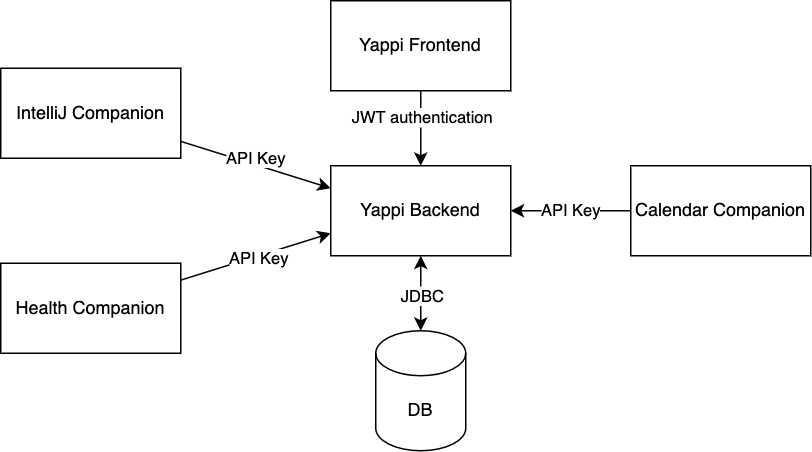
\includegraphics[width=0.95\textwidth]{../figures/plattform-system-diagram.drawio.png}
  \caption{Systemarchitektur der Yappi-Integrationsplattform}
  \label{fig:systemarchitektur}
\end{figure}

Das in Abbildung \ref{fig:systemarchitektur} dargestellte Architekturdiagramm zeigt die zentralen Komponenten der 
Yappi-Integrationsplattform sowie deren Anbindung an externe Companion-Anwendungen. Im Zentrum befindet sich das Yappi Backend,
das als zentrale Schnittstelle für alle eingehenden Daten und Anfragen fungiert.

Das Yappi Frontend verwendet die bestehende JWT-basierte Authentifizierung zur Verwaltung von Nutzersitzungen. Externe
Companion-Apps, wie beispielsweise die IntelliJ-, Health- oder Calendar-Companion, sind über einen API-Key-Mechanismus angebunden.
Dieser gewährleistet, dass nur registrierte und autorisierte Clients Daten an das System übermitteln können. Alle eingehenden
Daten werden vom Backend in der dargestellten Datenbank (DB) persistiert.

\subsubsection{Sicherheit}

Der API-Key-Mechanismus der Integrationsplattform ist so konzipiert, dass er eine sichere und kontrollierte Anbindung externer
Companion-Anwendungen ermöglicht. Jeder API-Key ist eindeutig einem Nutzerkonto zugeordnet und wird in der Webanwendung einmalig
generiert. Die Generierung erfolgt über eine abgesicherte Benutzeroberfläche, wodurch sichergestellt ist, dass ausschliesslich
berechtigte Nutzer einen Schlüssel anlegen können. Zur Übertragungssicherheit wird der API-Key ausschliesslich über verschlüsselte
Verbindungen (HTTPS) zwischen der Companion-Anwendung und dem Backend übertragen.

Im Backend erfolgt eine serverseitige Validierung, bei der der Schlüssel auf Gültigkeit und Zuordnung geprüft wird. Die Schlüssel
werden dabei nicht im Klartext gespeichert, sondern in sicherer Form (z. B. gehasht) abgelegt, um auch bei einem möglichen
Datenbankzugriff unbefugten Gebrauch zu verhindern. Ein kompromittierter API-Key kann jederzeit durch den Nutzer oder einen
Administrator gesperrt oder durch einen neuen ersetzt werden.

\subsubsection{Ablauf der API-Key Erstellung und -Verwendung}

Abbildung \ref{fig:apikey-swimlane} zeigt den Ablauf der Erstellung und Verwendung des API-Keys innerhalb der
Yappi-Integrationsplattform. Die Darstellung erfolgt als Swimlane-Diagramm und verdeutlicht die beteiligten Akteure sowie deren
Interaktionen während des gesamten Prozesses.

\begin{figure}[!htbp]
  \centering
  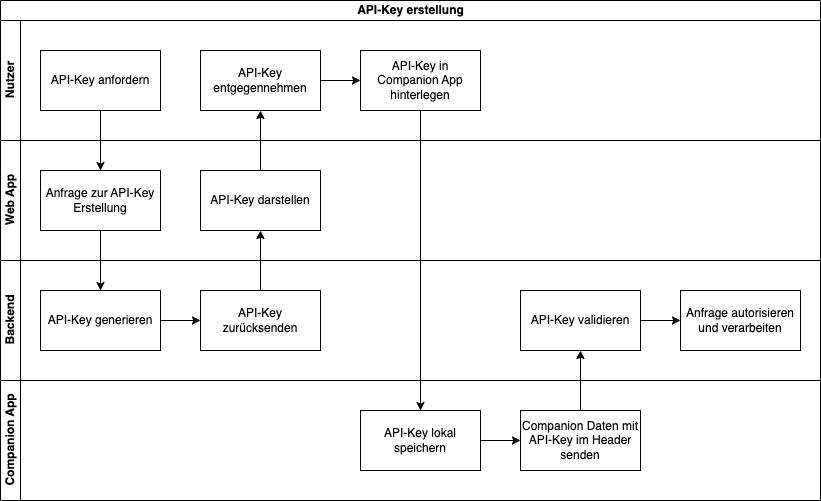
\includegraphics[width=0.95\textwidth]{../figures/apikey-swimlane-diagram.drawio.png}
  \caption{Ablauf der API-Key Erstellung und -Verwendung in Yappi}
  \label{fig:apikey-swimlane}
\end{figure}

Der Prozess beginnt mit der einmaligen Generierung des API-Keys durch den Nutzer in der Webanwendung. Nach der Erstellung wird der
Schlüssel in der Companion-App hinterlegt und dort dauerhaft gespeichert. Jede Datenanfrage der Companion-App an das Backend
enthält den API-Key im HTTP-Header, woraufhin das Backend den Schlüssel validiert und die Anfrage bei positiver Prüfung
autorisiert. Dieser Ablauf stellt sicher, dass ausschliesslich autorisierte Anwendungen im Namen eines Nutzers Daten an Yappi
übermitteln können.





\chapter{Implementierung}
\todo{Einleitung}

\section{Zugriffskontrolle über API-Keys}

    Das API-Key-System dient der sicheren und eindeutigen Authentifizierung externer Dienste gegenüber der \texttt{Yappi-Companion}-API.
    Anstelle von Benutzeranmeldedaten verwenden Clients einen statisch generierten API-Key, der für den jeweiligen Nutzer erstellt und ausschliesslich diesem zugeordnet ist.
    Dies ermöglicht den kontrollierten Zugriff auf geschützte Endpunkte, ohne dass sensible Login-Daten offengelegt oder dauerhaft gespeichert werden müssen.

    Über einen gültigen API-Key können autorisierte Clients Anfragen an Endpunkte mit dem Pfadpräfix \texttt{/companion/} stellen.
    Beispielsweise kann der Fragenblock mit der ID~\texttt{1} wie folgt abgerufen werden:

    \begin{verbatim}
        GET https://yappi.dev/companion/questionblocks/1
        X-API-KEY: <api-key>
    \end{verbatim}


    \subsubsection{Datenbank}
    Die Tabelle \texttt{api\_key} speichert die Metadaten und API-Keys.

    \begin{table}[!htbp]
    \centering
    \begin{tabular}{|l|l|p{9cm}|}
    \hline
    \textbf{Spalte} & \textbf{Datentyp} & \textbf{Beschreibung} \\
    \hline
    \texttt{id} & SERIAL & Primärschlüssel, auto-inkrementierend \\
    \texttt{user\_id} & INTEGER & Fremdschlüssel auf \texttt{users.id} \\
    \texttt{hashed\_key} & TEXT & Gesalteter Hash des API-Keys (z.\,B. BCrypt oder Argon2) \\
    \texttt{created\_at} & TIMESTAMPTZ & Zeitpunkt der Erstellung des Keys \\
    \texttt{expires\_at} & TIMESTAMPTZ & Optionales Ablaufdatum \\
    \texttt{active} & BOOLEAN & Aktivierungs-Flag, um Keys ohne Löschung zu sperren \\
    \hline
    \end{tabular}
    \caption{Schema der Tabelle \texttt{api\_key}}
    \label{tab:api_key_schema}
    \end{table}

    \subsubsection{Backend-Komponenten}
    \begin{itemize}
      \item \textbf{Entität} (\texttt{ApiKey.java}) - Abbildung der Tabelle \texttt{api\_key} als JPA-Entität, ohne Feld für den rohen Key.
      \item \textbf{Repository} (\texttt{ApiKeyRepository.java}) - Zugriff auf API-Key-Datensätze, inkl. Suche nach Key-Präfix.
      \item \textbf{Util-Klasse} (\texttt{ApiKeyUtil.java}) - Generierung zufälliger Keys, Trennung von Präfix und geheimem Teil, Hashing des geheimen Teils mit einem sicheren Algorithmus.
      \item \textbf{Service} (\texttt{ApiKeyService.java}) - Erstellung, Speicherung und Validierung von Keys.
      \item \textbf{Controller} (\texttt{ApiKeyController.java}) - REST-Endpunkte zur Verwaltung von Keys.
    \end{itemize}

    \subsubsection{API-Endpunkte}
    Basispfad: \texttt{/apikey}. Alle Endpunkte setzen einen gültigen JWT im \texttt{Authorization}-Header voraus (\texttt{Bearer <token>}).

    \begin{itemize}
      \item \texttt{GET /apikey} \\
            Liefert den aktiven API-Key des aktuell authentisierten Nutzers als Metadatenobjekt (kein Klartext-Key). \\
            \textbf{Antworten:} \texttt{200 OK}, \texttt{404 Not Found} (kein aktiver Key), \texttt{401 Unauthorized} (fehlender/ungültiger Header).
      \item \texttt{POST /apikey/generate} \\
            Erzeugt einen neuen API-Key für den authentisierten Nutzer und gibt den Klartext-Key einmalig zurück. \\
            \textbf{Antworten:} \texttt{200 OK}, \texttt{401 Unauthorized}.
    \end{itemize}

    \noindent
    \textbf{Nutzung geschützter Ressourcen:} Externe Clients authentisieren sich anschliessend mit \texttt{X-API-KEY: <key>} gegenüber den Companion-/Backend-Endpunkten. Der Klartext-Key wird nicht gespeichert; in der Datenbank liegt nur \texttt{hashed\_key}.

    \noindent
    \textbf{Beispiel (cURL):}
    \begin{verbatim}
    # Key erzeugen
    curl -H "Authorization: Bearer <JWT>" -X POST https://<host>/apikey/generate

    # Aktiven Key (Metadaten) abrufen
    curl -H "Authorization: Bearer <JWT>" https://<host>/apikey
    \end{verbatim}

    \subsubsection{Verarbeitungslogik}//
    \textbf{Erstellung:}
    \begin{enumerate}
      \item Generierung eines neuen Keys (Präfix + geheimer Teil).
      \item Hashing des geheimen Teils.
      \item Speicherung des Hashes und der Metadaten in der Tabelle \texttt{api\_key}.
      \item Rückgabe des vollständigen Keys an den Client (nur einmalig).
    \end{enumerate}
    \textbf{Validierung:}
    \begin{enumerate}
      \item Extraktion des Präfixes und geheimen Teils aus dem API-Key-Header.
      \item Abruf des Datensatzes anhand des Präfixes.
      \item Prüfung auf Existenz, Aktivstatus und Ablaufdatum.
      \item Vergleich des Hashes mit dem übergebenen geheimen Teil.
      \item Bei Erfolg: Authentifizierung des zugehörigen Benutzers.
    \end{enumerate}

    \subsubsection{Sicherheitsintegration}
    \begin{itemize}
      \item \textbf{ApiKeyFilter} - Spring-Security-Filter, der den API-Key aus dem \texttt{X-API-KEY}-Header ausliest und validiert.
      \item \textbf{SecurityConfig} - Bindet den Filter vor dem \texttt{UsernamePasswordAuthenticationFilter} in die Filterkette ein, um API-Key-Anfragen vor anderen Authentifizierungsmethoden zu prüfen.
    \end{itemize}

    \subsubsection{Vorteile}
    \begin{itemize}
      \item Schlüssel werden nie im Klartext gespeichert.
      \item Flexible Verwaltung durch Ablaufdaten und Aktivierungs-Flag.
      \item Sichere Hashing-Verfahren verhindern Missbrauch bei Datenbankkompromittierung.
    \end{itemize}


    \todo{Quelle für spring Securtiy Architektur}
    https://docs.spring.io/spring-security/reference/servlet/architecture.html \\
    \todo{Security "Workarround" erklären}
    \todo{Front End Anpassung}

\printbibliography

\end{document}
